\documentclass[12pt]{article}

\usepackage[utf8]{inputenc}
\usepackage[T2A]{fontenc}
\usepackage[english]{babel}
\usepackage{amssymb}
\usepackage{graphicx}
\usepackage{float}
\graphicspath{ {images/} }

\textwidth=431pt
\textheight=600pt
\hoffset=-15pt
\voffset=-15pt

\usepackage{graphicx}
\usepackage{amsmath}
\makeatletter
\renewcommand{\@oddhead}{%
\vbox{%
\hbox to \textwidth{\strut \textit{CV, Assignment 2, Usvyatsov Mikhail} \hfill }
\hrule
\vspace{12pt}
}}
\renewcommand{\@oddfoot}{}
\makeatother

\begin{document}
	\bigskip
	\textbf{Algorithm}
	
For every image we have to analyze it.
	
For each sample image we:\\

	\begin{enumerate}
		\item Clear the noise with Gaussian filter;
		\item Convert image to grayscale;
		\item Extract edges with Canny;
		\item Split image to images of every bottle;
		\item Extract the body of the bottle;
		\item Delete small contours from the bottle;
		\item With counting median intensity we can understand whether it has a label or not
		\item If it has a label, compute average distances from the bottle border to the label of contour from the left side and from the right side.
		\item If left distance in average is the same as right distance, than it is centered
		\item If all the distances are constant, it means, that label is straight. 
	\end{enumerate}
	
	\textbf{Illustration}
	
	Here are a few results of image processing:\\
	
	\begin{figure}[H]
		\centering
		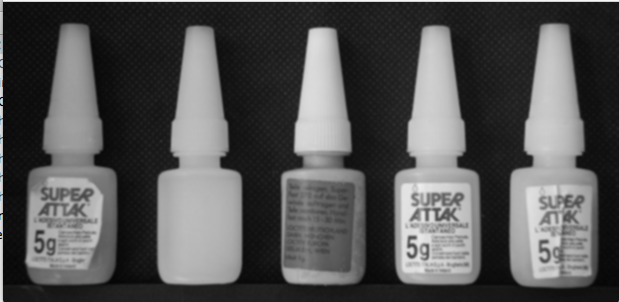
\includegraphics[width=15cm]{1}
		\caption{"Grayscaled image"}
	\end{figure}
	
	\begin{figure}[H]
		\centering
		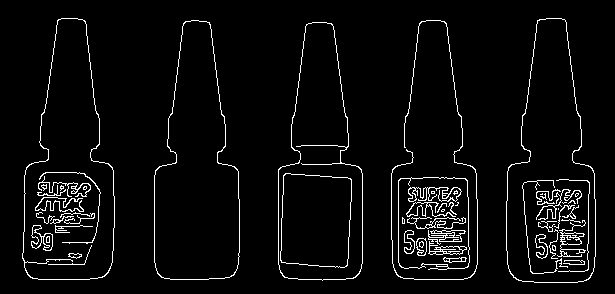
\includegraphics[width=15cm]{2}
		\caption{"Edges"}
	\end{figure}
	
	\begin{figure}[H]
		\centering
		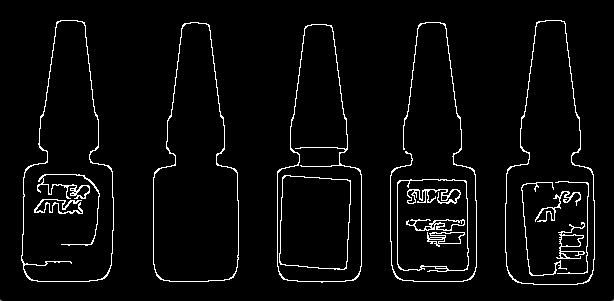
\includegraphics[width=15cm]{3}
		\caption{"Filtered edges"}
	\end{figure}
	
	\begin{figure}[H]
		\centering
		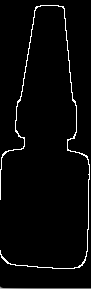
\includegraphics{4}
		\caption{"Extracted bottle"}
	\end{figure}
	
	\begin{figure}[H]
		\centering
		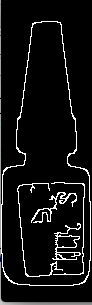
\includegraphics{5}
		\caption{"Another extracted bottle"}
	\end{figure}
	
	\begin{figure}[H]
		\centering
		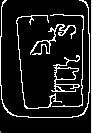
\includegraphics{6}
		\caption{"Extracted body"}
	\end{figure}
	
	\medskip
	
	\textbf{Performance measure}
	According to confusion matrix:
	
	\begin{tabular}{|c||c|c|c|}
		\hline
		\ & predicted 1 & predicted 0 & Total \\
		\hline
		real class 1 & True Positive (TP) & False Negative (FN) & P\\
		\hline
		real class 0 & False Positive (FP) & True Negative (TN) & N \\
		\hline
		Total & $P'$ & $N'$ & $P+N$\\
		\hline 
	\end{tabular}
	\medskip
	
	The formulas for precision, recall and accuracy:
	\newcounter{ecounter}
	\begin{list}{\arabic{ecounter})~}{\usecounter{ecounter}}
		\item $precision = \dfrac{TP}{TP+FP}$
		\item $recall = \dfrac{TP}{P}$
		\item $accuracy = \frac{TP+TN}{P+N}$
	\end{list}
	
	The results of the program:

	precision = recall = accuracy = 100%
	
\end{document}